\newpage
\section*{Написание скриптов на bash. Математические вычисления.}
	\paragraph*{1) Скрипт для отображение чисел Фибоначи от 0 до N для заданного N,
		 при N $\in$ $\R$\\ \\}

		На рисунке 1 изображено окно текстового редактора \textit{sublime}.\\

		\textbf{Небольшое пояснение к коду:\\}

		\textit{\#!/bin/bash} указывает путь к интерпретатору для исполнения скрипта.\\
		
		\textit{printf} - команда перекочевавшая из языка \textit{C}, более продвинутый аналог \textit{echo} для вывода сообщения в стандартное устройство вывода.
		В качестве парметров принимает 'формат вывода' 'Тест для вывода'\\

		Номер, до которого нужно вычислять последовательность чисел Фибоначи получаем из первого параметра при запуске скрипта. Он хранится в переменной \textit{\$1}\\

		В программе спользуется цикл \textit{for} для контроля номера числа Фибоначи. В качестве начальных известных значений чисел Фибоначи взяты первые три числа.\\

		С помощью оператора потокового вывода >> результат работы скрипта сохраняем в файл \textit{fibi.data}\\
		Результат работы скрипта и вывод содержимого файла \textit{fibi.data} можно увидеть на Рисунке 2.\\

		\vspace{0.5cm}
		\begin{center}
			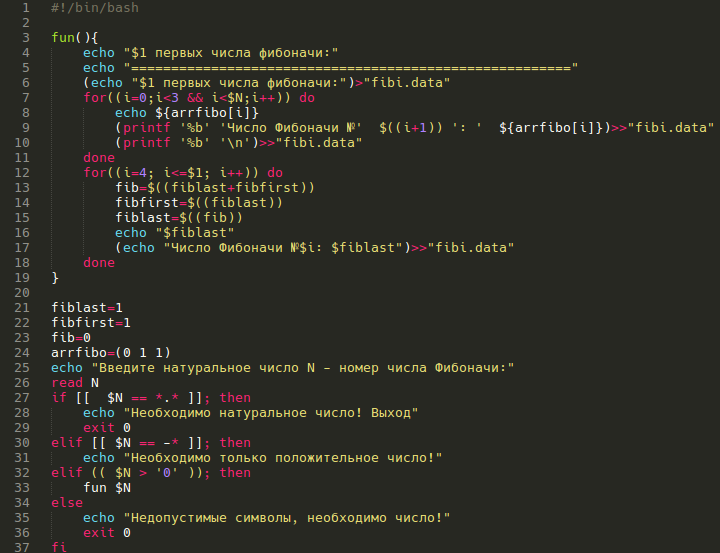
\includegraphics[width=\textwidth]{fibo.png}
			Рисунок 1 - скрипт для вычисления последовательности Фибоначи от 0 до N\\

			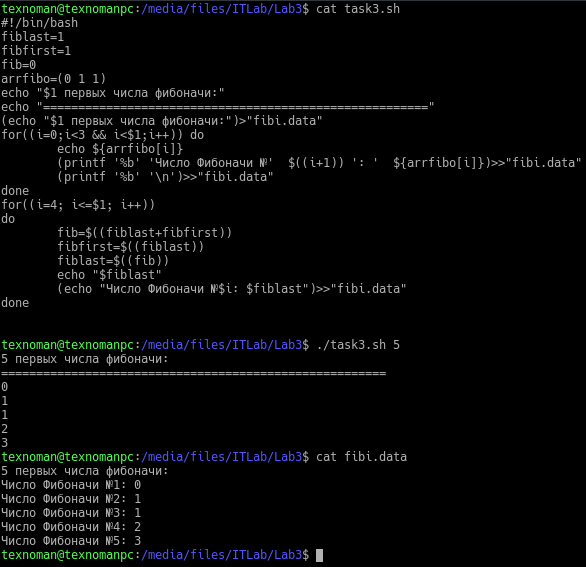
\includegraphics[width=\textwidth]{fiboT.png}
			Рисунок 2 - результат работы скрипта по поиску чисел Фибоначи, \\ 
			вывод содержимого скрипта и вывод содержимого файла, храняшего результат работы скрипта.\\
		\end{center}

	\vspace{1cm}
	\paragraph{2)Скрипт вычисляющий факториал N для заданного N, при N $\in$ $\R$\\ \\}
		На рисунке 3 изображено окно того же текстового редактора \textit{sublime}, показывающее код программы.\\

		\textbf{Пояснение к коду:\\}

		\textit{\#!/bin/bash} все также указывает путь к интерпретатору для исполнения скрипта (bash).\\
		
		Команда \textit{let} производит арифметические операции над числами и переменными, в данном случае умножение на число и одновременное присвоение ему нового значения (\textit{*=}). Оператор разыменования переменной \textit{\$} для \textit{let} не нужен.\\

		Данный скрипт считает факториал для заданного в качестве параметра при исполнении числа N.\\

		С помощью оператора потокового вывода > (перезаписывает файл) результат работы скрипта сохраняем в файл \textit{factor.data}.\\

		Результат работы скрипта и вывод содержимого файла \textit{factor.data} можно увидеть на Рисунке 2.\\

		\vspace{0.5cm}
		\begin{center}
			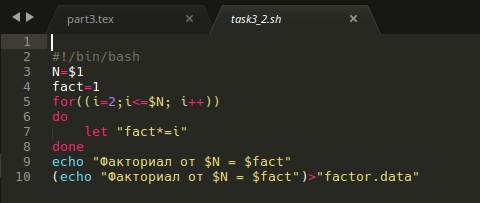
\includegraphics[width=\textwidth]{fact.png}
			Рисунок 3 - скрипт для вычисления факториала для числа N\\

			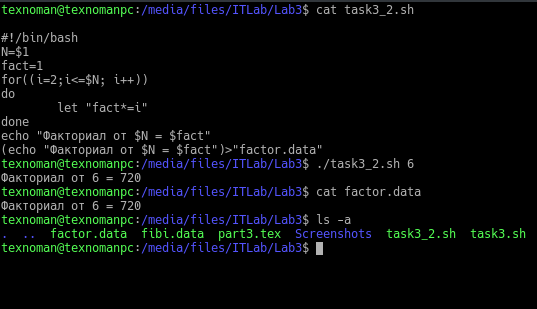
\includegraphics[width=\textwidth]{factT.png}
			Рисунок 4 - результат работы скрипта по поиску факториала числа N, \\ 
			вывод содержимого скрипта и вывод содержимого файла, хранящего результат работы скрипта.\\
		\end{center}